\documentclass{beamer}

\usepackage[utf8]{inputenc}
\usepackage{graphicx}
\usetheme{Copenhagen}
\usecolortheme{default}
\usepackage{media9}
\renewcommand{\figurename}{Slika}

%Information to be included in the title page:
\title[Optimizacija rojem čestica]{Optimizacija rojem čestica}
\author{Nevena Soldat, Tijana Živković, Ana Miloradović, Milena Kurtić}
\institute{Matematički fakultet, Univerzitet u Beogradu}
\date{\today}



\begin{document}
\frame{\titlepage}

\begin{frame}
\frametitle{Pregled}
\begin{itemize}
    \item{Uvod u optimizaciju rojem čestica}
    \item{Osnovni algoritam}
    \item{Varijacije parametara}
    \item{Primena}
    \item{Topologije}
    \item{Literatura}
\end{itemize}

\end{frame}

\begin{frame}{Uvod}

Šta je optimizacija rojem čestica?
\begin{itemize}
    \item optimizaciona tehnika zasnovana na inteligentnom ponašanju nekih organizama, kao što su insekti, ptice i ribe

\end{itemize}

Nastanak:
\begin{itemize}
    \item Eugene Marais - The Soul of the White Ant (1926)
    \item Marco Dorigo - ponašanje kolonije mrava (1990-ih) 
    \item Eberhart i Kennedy - algoritam optimizacije rojem čestica (1995)
\end{itemize}

Algoritam za optimizaciju rojem čestica je otkriven sasvim slučajno, pri pokušaju da se na računaru simulira kretanje jata ptica.
\end{frame}

\begin{frame}{Osnovni algoritam}
Osnovni koncepti:
\begin{itemize}
    \item čestice se kreću kroz višedimenzioni prostor pretrage
    \item svaka čestica predstavlja jedno moguće rešenje
\end{itemize}

Neka je $x_i(t)$ pozicija čestice \textit{i} u trenutku \textit{t}. Pozicija se menja dodavanjem brzine $v_i(t)$ na trenutku poziciju:
\[ x_i(t+1) = x_i(t) + v_i(t+1) \]
Brzina se računa kao:
\[ v_i(t+1) = v_i(t) + c_1r_1(p_i(t) - x_i(t)) + c_2r_2(p_g(t) - x_i(t))\] gde su:

\begin{itemize}
    \item $p_i(t)$ - najbolja pozicija koju je čestica \textit{i} pronašla do trenutka \textit{t}
    \item $p_g(t)$ - najbolja pozicija u čitavom roju do trenutka \textit{t}
    \item $r_1, r_2$ - nasumične vrednosti iz \textit{U}[0,1]
    \item $c_1, c_2$ - konstante
\end{itemize}

\end{frame}


\begin{frame}{Komponente brzine}
    \begin{figure}[htp]
    \centering
    \includegraphics[scale = 1.2]{velocity.png}
    \caption{Komponente brzine}
    \label{fig:velocity}
\end{figure}

\begin{itemize}
    \item \textbf{moment} - prethodno stanje brzine
    \item \textbf{kognitivna} komponenta - tendencija vraćanja u lično najbolje
    \item \textbf{socijalna} komponenta - tendencija ka kretanju ka naboljem globalnom
\end{itemize}
\end{frame}

\begin{frame}{Osnovne varijacije: Smanjenje brzina}
Modifikacije osnovnog algoritma optimizacija rojem čestica

\begin{itemize}
    \item \textbf{Eksploracija} - istraživanje različitih delova prostora pretrage
    \item \textbf{Eksploatacija}  -  koncentrisanje oko regije koje garantuje nalaženje rešenja
\end{itemize}
Smanjenje brzina uvodi se da bi se sprečilo da čestice napuste  prostor pretrage usled čestog ažuriranja položaja


\begin{equation}
    v_i(t+1) = \begin{cases}
                
            v'_i(t+1),  &  v'_i(t+1) < V_{max}\\
            V_{max},  &   v'_i(t+1) \geq V_{max}
           
             \end{cases}
\end{equation}

\end{frame}

\begin{frame}{Osnovne varijacije: Inercijske težine}
U osnovnu formulu ažuriranja brzine uvodi se težina $w$ koji konroliše koliko će prethodni pravac leta uticati na novu brzinu, kao i sam balans između istraživanja i eksploatacije
\[v_{ij}(t+1) = wv_{ij}(t) + c_1r_{1j}(t)[y_{ij}(t) - x_{ij}(t)] + c_2r_{2j}(t)[\hat{y}_{ij}(t) - x_{ij}(t)] \]

Veće vrednosti $w$ olakšavaju eksploraciju, dok manje vrednosti $w$ podstiču lokalnu eksploataciju

\begin{itemize}
    \item $w$ $>=$ 1 - roj divergira, brzine idu ka maksimalnoj brzini
    \item 0 $<$ $w$ $<$ 1  -  čestice usporavaju, pa konvergencija zavisi od $c_1$ i $c_2$
    \item $w$ $<$ 0 -  brzine opadaju sve dok ne stignu do nule i time se algoritam zaustavlja
\end{itemize}

\end{frame}

\begin{frame}{Osnovne varijacije: Koeficijent suženja i model brzine}

Ovaj princip je sličan inercijskoj težini, ali se brzine ograničavaju konstantom $\chi$

\[v_{ij} (t + 1) = \chi[v_{ij} (t) + \phi_1 (y_{ij} (t) - x_{ij} (t)) + \phi_2 (\hat{y}_j (t) - x_{ij} (t))]\]
gde je $$\chi = \frac{2k}{|2-\phi-\sqrt{\phi(\phi-4)}|},$$sa $\phi = \phi_1 +  \phi_2 , \phi_1 = c_1r_1$ i $\phi_2 = c_2r_2$\

Modeli brzina se razlikuju u komponentama koje su uključene u jednačinu brzine
\begin{itemize}
    \item \textbf{Kognitivni} model - isključuje socijalnu komponentu
    \item \textbf{Socijalni} model- isključuje kognitivnu komponentu
    \item model u kojoj sama \textbf{čestica neće sebe izabrati za najbolju} - najbolje rešenje se bira iz susedstva
    
\end{itemize}

\end{frame}

\begin{frame}{Primene}

\frametitle{Primene}
\begin{itemize}
\item Kontinualni i diskretni problemi
\item \textbf{Oblasti primene:} Neuronske mreže, telekomunikacije, istraživanje podataka, dizajn(antene, bluetooth), kombinatorna optimizacija, biomedicina itd.
\item Šta je \textbf{distributivna mreža}?
\begin{itemize}
    \item deo elektroenergetskog sistema koji omogućava da se električna energija distribuira do srednjih i malih potrošača. 
\end{itemize}
\item \textbf{Proces planiranja} razvoja distributivnih mreža:
\begin{itemize}
    \item Šta?
    \item Gde? 
    \item Kada?
\end{itemize}

\end{itemize}


\end{frame}


\begin{frame}{Primene}

\frametitle{Primene}
\begin{itemize}
\item \textbf{Formulacija problema} 
\begin{itemize}
    \item \textbf{Faktori} - minimizacija gubitaka energije, ulaganja u nove objekte i distributivne vodove, maksimizacija pouzdanosti sistema
    \item \textbf{Ograničenja} - kapacitet vodova, naponski nivo opterećenja u čvorovima, radijalnost mreže
    \item \textbf{Funkcije cilja} - gubitak energije, pouzdanost sistema
\end{itemize}
\item \textbf{Šema kodiranja čestica} - kodira topologiju mreže, direktno i indirektno kodiranje
\item \textbf{Šema dekodiranja čestica} - troškovno pristrasno dekodiranje

\end{itemize}


\end{frame}


\begin{frame}{Primene}
\begin{figure}
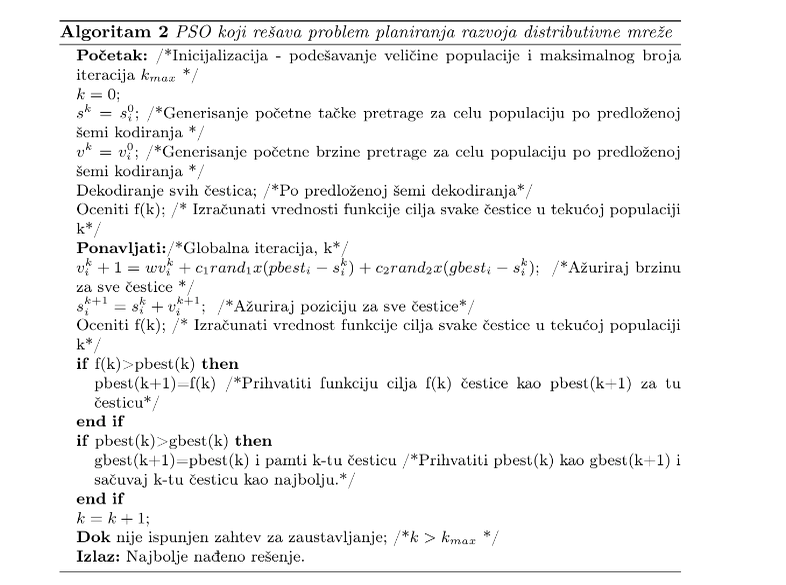
\includegraphics[scale=0.3]{distPSO.png}
\end{figure}

\end{frame}

\end{document} 
